%---------------DOCUMENT SETTINGS------------------------------------
%\documentclass{article}
\documentclass[
    paper=A4,					% paper size --> A4 is default in Germany
    twoside=true,				% onesite or twoside printing
    openright,					% doublepage cleaning ends up right side
    parskip=full,				% spacing value / method for paragraphs
    chapterprefix=true,			% prefix for chapter marks
    11pt,						% font size
    headings=normal,			% size of headings		% include listof entries in toc
    titlepage=on,				% own page for each title page
    captions=tableabove,		% display table captions above the float env
    draft=false,
]{scrreprt}
\usepackage[english]{babel}
\usepackage{wrapfig}
\usepackage[utf8]{inputenc} % utf8x durch utf8 ersetzt wegen biblatex
\usepackage[T1]{fontenc}
\usepackage{amsmath,amssymb,amstext,amsfonts}

\usepackage{csquotes}
\usepackage{pdfpages} %zum importieren des Deckblattes
\usepackage{geometry}
\usepackage[headsepline]{scrlayer-scrpage}
\usepackage{lastpage}
%Literaturverwaltung
\usepackage{tabularx} %für die Legende im Gruundlagen Oszi Bild
\usepackage{tabulary}
\usepackage{float}
\usepackage{textcomp}
\usepackage{gensymb}
\usepackage{physics}
\usepackage{stmaryrd}
\usepackage{graphicx}
\usepackage[export]{adjustbox}
\usepackage{a4wide}
\usepackage{siunitx}
\usepackage{hyperref}
\usepackage{multicol}
\usepackage{makecell}
\usepackage{enumitem}
\usepackage{subcaption}


%\geometry{      %holt mehr aus einer A4 Seite raus
%    a4paper,
%    total={170mm,257mm},
%    left=20mm,
%    top=25mm,
%   }
\graphicspath{ {./graphics/} }  %pfad für bilder
\hypersetup{colorlinks=false}
%\addbibresource{literatur.bib} %Literatur-Resourcen\s
%\setlength{\headheight}{0.0pt} % macht zwar headheight warnings aber dafür nutz latex die seitengröße besser aus.
\pagestyle{scrheadings}
\newcommand{\subf}[2]{
    {
        \begin{tabular}[c]{@{}c@{}}
            {\setlength{\extrarowheight}{100pt} #1 }\\#2
        \end{tabular}
    }
}
\newcommand{\allc}{\multicolumn{1}{c|}{-}}
\newcommand{\monofig}[4]{
    
    \begin{figure}[H]
    \centering
    \includegraphics[#1]{#2}
    \caption{
        #3
    }
    \label{#4}
    \end{figure}
    
}
\newcommand{\polyfig}[6]{
    \begin{figure}[H]
        \centering
        \begin{minipage}[b]{0.45\textwidth}
            \centering
            \includegraphics[width=\textwidth]{#1}
            \caption{#2}
            \label{#3}
        \end{minipage}
        \begin{minipage}[b]{0.45\textwidth}
            \centering
            \includegraphics[width=\textwidth]{#4}
            \caption{#5}
            \label{#6}
        \end{minipage}
    \end{figure}
}
\newcommand{\polyfigacc}[8]{
    \begin{figure}[H]
        \centering
        \begin{minipage}[b]{#1}
            \centering
            \includegraphics[width=\textwidth]{#2}
            \caption{#3}
            \label{#4}
        \end{minipage}
        \begin{minipage}[b]{#5}
            \centering
            \includegraphics[width=\textwidth]{#6}
            \caption{#7}
            \label{#8}
        \end{minipage}
    \end{figure}
}
\newcommand{\trifig}[9]{
    \begin{figure}[H]
        \centering
        \begin{minipage}[b]{0.32\textwidth}
            \centering
            \includegraphics[width=\textwidth]{#1}
            \caption{#2}
            \label{#3}
        \end{minipage}
        \begin{minipage}[b]{0.32\textwidth}
            \centering
            \includegraphics[width=\textwidth]{#4}
            \caption{#5}
            \label{#6}
        \end{minipage}
        \begin{minipage}[b]{0.32\textwidth}
            \centering
            \includegraphics[width=\textwidth]{#7}
            \caption{#8}
            \label{#9}
        \end{minipage}
        \caption{#10}
        \label{#11}
    \end{figure}
}

\date{\today{}, Location}
\author{Aleksey Sokolov, Max Jost}
\title{Wirkungsgrad}

%---------------HEADER TEXT------------------------------------
\clearpairofpagestyles
\ihead{\today{} \\ }
\chead{Max Jost / Aleksey Sokolov\\ Wirkungsgrad }
\ohead{FPTP 2 \\ }
\cfoot{\pagemark \, / \, \pageref{LastPage}}

%---------------DOCUMENT TEXT------------------------------------
\newpairofpagestyles{chapteropening}{%
    \cfoot{\pagemark \, / \, \pageref{LastPage}} % Display chapter name and page number
}

% Modify the chapter command to use the custom page style
%\renewcommand*{\chapterpagestyle}{chapteropening}



%---------------DOCUMENT TEXT------------------------------------
\begin{document}
%
\includepdf[]{Deckblatt.pdf} %Insert title page NaWi-Graz
%\pagestyle{maincontentstyle}

\chapter*{Abstract}
\label{sec:abstract}


\tableofcontents
\newpage
%***************ANMERKUNGEN*******************
\chapter{Introduction}
\label{sec:anmerkung}
Since the development of the Scanning Tunneling Microscope (STM) in 1981 it was used to get an Insight in to electronic structure of molecules and individual atoms in crystals.
Especially the adsorbtion of organic molecules on metal or metal-oxide substrates peaked interest in the STM-Imaging Field in recent years.
The reason why there is a lot of interest in studying these organic adsorbents is their promissing semiconducting properties and their capacity for self-assembly.
Additionally they promise cheap, flexible and tunable alternatives to conventional metal-semiconducters in electronic and optoelectronic \cite{OTERO2017105}.

%********VORAUSSETZUNGEN & GRUNDLAGEN*********
\chapter{Fundumentals}
\label{sec:Fundumentals}
\section{STM-Imaging}
The Scanning Tunneling Microscope was introduced in 1981 by Gerd Binning and Heinrich Roherer. 
With this measuring technique it is possible to resolve a conductive surface with a precission beyond that of conventional light based Microscopes.
In contrast to other electron based microscopy like Scanning Electron Microscopes (SEM) it uses the quantum mechanical phenomenon of tunneling.
In classical mechanics, objects cannot overcome a potential if their energy $E < V_0$, as observed in gravitational interactions.
This phenomenon is observed for quantum mechanical particles like electrons, which can surpass a potential barrier despite the initial expectation that they should not be able to.
The STM uses this effect by precisely positioning a sharp conductive tip close to the surface and applying a bias voltage.
Most STM are operated in Ultra-High-Vacuum (UHV), where the distance between the tip and the surface represents the tunneling barrier.
By varying the bias voltage, the tunneling probability can be changed, thereby affecting the tunneling current.
If the bias voltage, also referred to as the potential difference, is kept constant, the tunneling current is primarily dependent on the distance between tip and surface.
The tip is moved in the x-,y-plane where a grid is established. 
There are two modes of operation, the constant-height and the constant-current mode.
The latter is especially useful for irregular surfaces, because the tip is moved up and down to keep the tunneling current constant.
The movement signal of the piezos is then converted into height.
In constant-height mode the position of the tip stayes fixed and the tunneling current $I_t$ is measured and converted into height information. \\

\newpage
\begin{wrapfigure}{r}{0.5\textwidth}
    \centering
    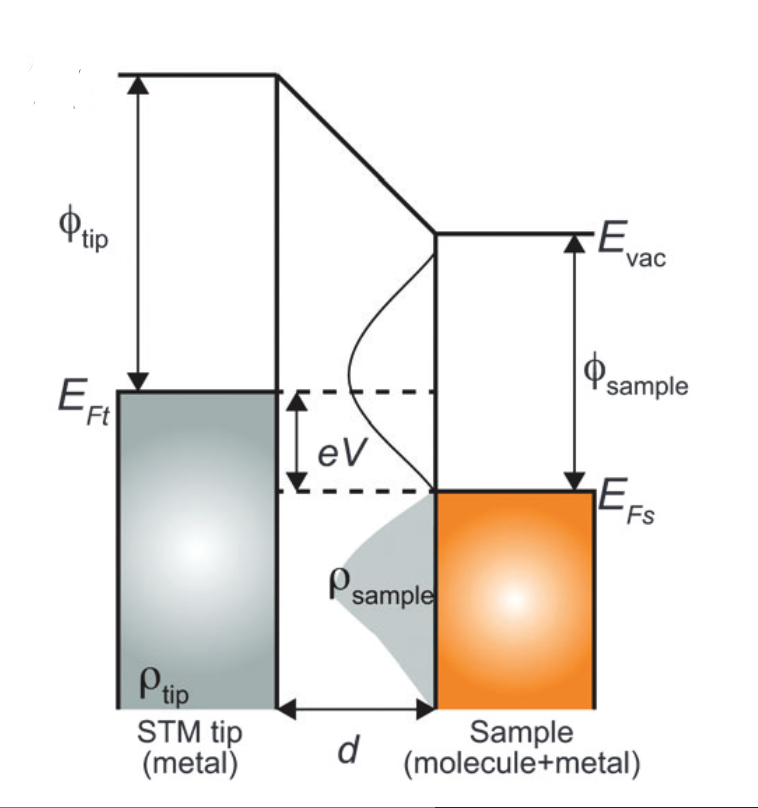
\includegraphics[width=0.4\textwidth]{graphics/Tunneling_diagram_japan.PNG}
    \caption{Energy diagram of the tunneling junction with a positive bias voltage applied. $\Phi_{tip}$ \& $\Phi_{sample}$: working functions of either tip and sample, $E_{vac}$: vacuum energy level,  $E_{ft}$ \& $E_{fs}$: Fermi Energys of the tip and sample,  $\rho_{tip}$ \& $\rho_{sample}$: density of states of tip and sample,  $eV$: potential difference caused by applying a bias Voltage $V$ (picture source: \cite{Kano}) }
    \label{fig:energy_diagram}
\end{wrapfigure}

The tunneling current, at a arbituery gridpoint, is influenced by the electronic structure of the tip and sample.
If the tip is in vicinity of the metallic substrate the fermi energies align, resulting in an equal probability of electrons tunneling from the tip to the sample and vice versa.
This consequently results in a zero net current. 
Through the introduction of a electric potential $V_{bias}$ the fermi energies of tip and sample can be shifted relative to each other (Figure \ref{fig:energy_diagram}).
If the bias voltage is positive the fermi energy of the sample is pushed down and electrons from occupied states in the tip can tunnel into the empty states of the sample.
Consequently if the bias voltage is negative electrons from the filled states of the sample tunnel into the tip.
The tunneling current is influenced by the distance $d$ between orbitals of the tip and the sample, which makes it possible to gain information about the electronic structure of the sample.
This is not really a representation of the real structure of the atoms or molecules, but the Local Density of States (LDOS) of the sample´s surface.
Utilizing this in Scanning Tunneling Spectroscopy (STS) provides additional information beyond the sample's topography.
Such as the chemical composition, bonding, the energy gap and band-bending effects \cite{cbai}.
\newpage
\section{Mathematical Foundation STM}
\begin{wrapfigure}{r}{0.3\textwidth}
    \centering
    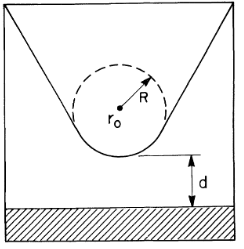
\includegraphics[width=0.3\textwidth]{graphics/fundamental_tip_sheme.PNG}
    \caption{Schematic depiction of the tip geometry \cite{PhysRevLett}}
    \label{fig:tip_scheme}
\end{wrapfigure}
To understand the tip sample interaction one must look at the quantum-mechnical Foundation behind it.
At its simplest the tip can be approximatated as spherical potential well (Figure \ref{fig:tip_scheme}). $R$ is in that case the radius of the tip located at position $\vec{r_0}$ with the distance $d$ from the surface.
First order pertubation theory gives the following expression (Eq. \ref{eq:tunneling_pert}) for the tunneling current of this system \cite{PhysRevLett}:
\begin{equation}
    I = \frac{2 \pi e}{\hbar} \sum_{\mu \nu} f(E_{\mu})[1 - f(E_{\nu}+eV_{bias})]\cdot |M_{\mu \nu}|^2 \delta(E_{\mu}- E_{\nu})
    \label{eq:tunneling_pert}
\end{equation}


The fermi distribution $f(E)= (\exp((E-E_F)/k_b T)+1)^{-1}$ gives the ocupation probability of a fermion (electrons) with the Energy $E$ near the fermi level.
In this case it is the ocupation probability of the tip states (denoted by the subindex $\mu$) and the ocupation probability of the sample states ( denoted by the subindex $\nu$).
The tunneling matrix $M_{\mu \nu}$ is related to the derivatives of the sample wave functions $\psi_{\nu} $ at the nucleus of the apex atom \cite{tunnelmatrix}.
Because the STM Imaging is done at low temperatures and with small voltages the Equation \ref{eq:tunneling_pert} can be simplified to:
\begin{equation}
    I = \frac{2 \pi}{\hbar} e^2 V_{bias} \sum_{\mu \nu}  |M_{\mu \nu}|^2 \delta(E{\nu}-E_F) \delta(E_{\mu}- E_{F})
    \label{eq:tunneling_pert_simple}
\end{equation}

\newpage

\section{Low Energy Electrons Diffraction (LEED)}
A well collimated beam of electrons with the same energy and thus the same wavelengh is directed ath a flat surface.
In this case the wavelengh of the incoming electrons is determened by the electric field $U_a$ that acts upon them \ref{eq:electron_wavelengh}.
To see diffraction the wavelengh of the electrons must be in the range of the lattice constant, as is effectively show by the concept of the ewald sphere.
Typically the kinetic energy of the electrons is up to $E_{kin} = e U_a = 200$ eV.
\begin{equation}
    \lambda = \frac{h}{\sqrt{2 m_e e U_a}}
    \label{eq:electron_wavelengh}
\end{equation} 
If the surface is periodic this results in a sharp pattern of spots that reflects the k-space of the crystal.

\begin{wrapfigure}{r}{0.6\textwidth}
    \centering
    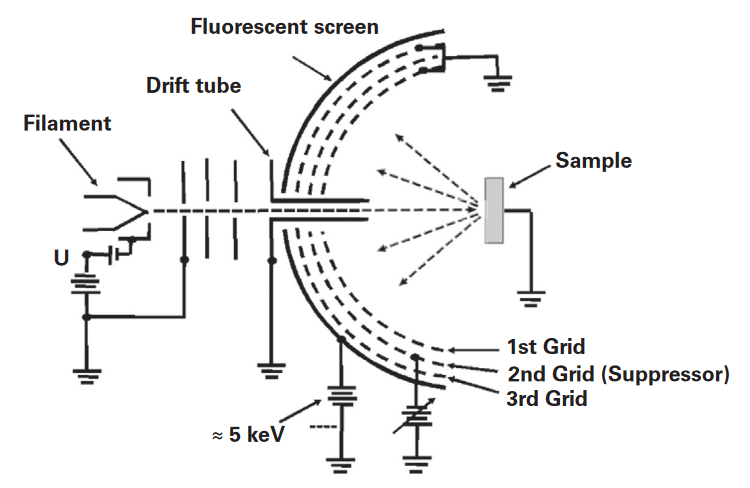
\includegraphics[width=0.5\textwidth]{graphics/fundamental_leed_setup.PNG}
    \caption{A basic three-grid LEED system which utilizes a flourenscent screen as imaging tool \cite{MoritzWolfgang2022SSDb}}
    \label{fig:LEED_Shematics}
\end{wrapfigure}

\noindent The LEED setup consists of a filament which emitts electrons by applying a current.
This electrons are then accelerated and collimated in a drift tube which points at the sample.
Due to interactions of the electrons with the crystal atoms some of them are not diffracted elastically.
To ensure that only the elastically scattered electrons are show on the flourencent screen, a grid system is installed in front of the screen.
The first grid and the sample are both grounded to ensure that the diffracted alectrons propagate undesturbed through the space between the sample and the grid.
A filter Voltage is aplied between the second and third grid that is just below the acceleration voltage.
Electrons which are not elastically scattered are completely stopped, which makes it effectivelly a high pass filter. \cite{MoritzWolfgang2022SSDb} \\

\noindent The collimated beam can be represented as a planar wave $e^{i \vec{k_0} \vec{r}}$  outside the surface.
The wavevector $\vec{k_0}$ points in the propagation direction and represents the spacial frequency of the wave.
This vector can be modeled as:
\begin{align}
    |\vec{k_0}| &= \frac{2 \pi}{\lambda} = \frac{\sqrt{2 m_e E}}{\hbar} \\
    \hspace{1cm} \notag \\
    \vec{k_0} &= \begin{pmatrix}
        |k_0|\cos(\varphi)\sin(\vartheta)\\|k_0|\sin(\vartheta)\sin(\vartheta)\\|k_0| \cos(\vartheta)
    \end{pmatrix}
\end{align}
A 2D periodic surfuce structure with a reciprocal basis ($b_1$,$b_2$) causes the plane waves to diffract.
The diffracted waves have the shape $A_g e^{i \vec{k_g} \vec{r}}$ with wave vectors $|\vec{k_g}| = |\vec{k_0}|$.
$\vec{k_g}$ transforms according to $\vec{k_g} = \vec{k_0} + \vec{g}$. 
The reciprocal lattice vector $\vec{g} = 2 \pi ( h b_1 + k b_2)$ represents the individual points where constructive interference is present.
Usually the indices h and k are intergers which characterize the beam, for example (0,0) or (1,1).
It can be shown that the wave vector in vacuum outside the surface is \cite{MoritzWolfgang2022SSDb}:
\begin{equation}
    k_g = - \sqrt{\frac{2 m_e E}{\hbar^2} - (k_{0x}+ g_{x})^2 - (k_{0y}+ g_{y})^2}
\end{equation}

\polyfig{graphics/fundamental_kspace.PNG}{hi}{fig:kspace}{graphics/fundamental_kspace_heta.PNG}{fig:kspace2}{helo}
%************VERSUCHSANORDNUNG*************
\chapter{Experimental Setup}
\label{sec:versuchsandordnung}
The experimental work done in this thesis primarily utilized a Low-Temperature Scanning Tunneling Microscope setup (LT-STM).
This STM is composed of two distinct compartments, the preparation chamber (PC) the measurement chamber (MC).
The sample is inserted through a airlock into the preparation chamber.
In the whole system there is in a Ultra High Vacuum (UHV) at about 10$^{-11}$ - 10$^{-10}$ mbar, which is archieved by four individuall pumps.
The base Vacuum is achieved with the turbomolecular pump and the scroll pump through the airlock.
Additionally there is a titanium sublimation pump and a ion pump in the preparation room.

\monofig{width=\textwidth}{Experimental_Setup/STM_Picture_1_edited.pdf}{
    The experimental setup used, 
    A: cooling-chamber filled with Liquid Oxigen,
    B: measuring-chamber with spring suspended sample holder and tip,
    C: sputter-gun,
    D: metal-evaporater,
    E: molecule-evaporater,
    F: preparation-chamber with free movable sample holder arm,
    G: LEED system,
    H: Electronic used to monitor the function of the STM}{fig:stm_uni_kf}
%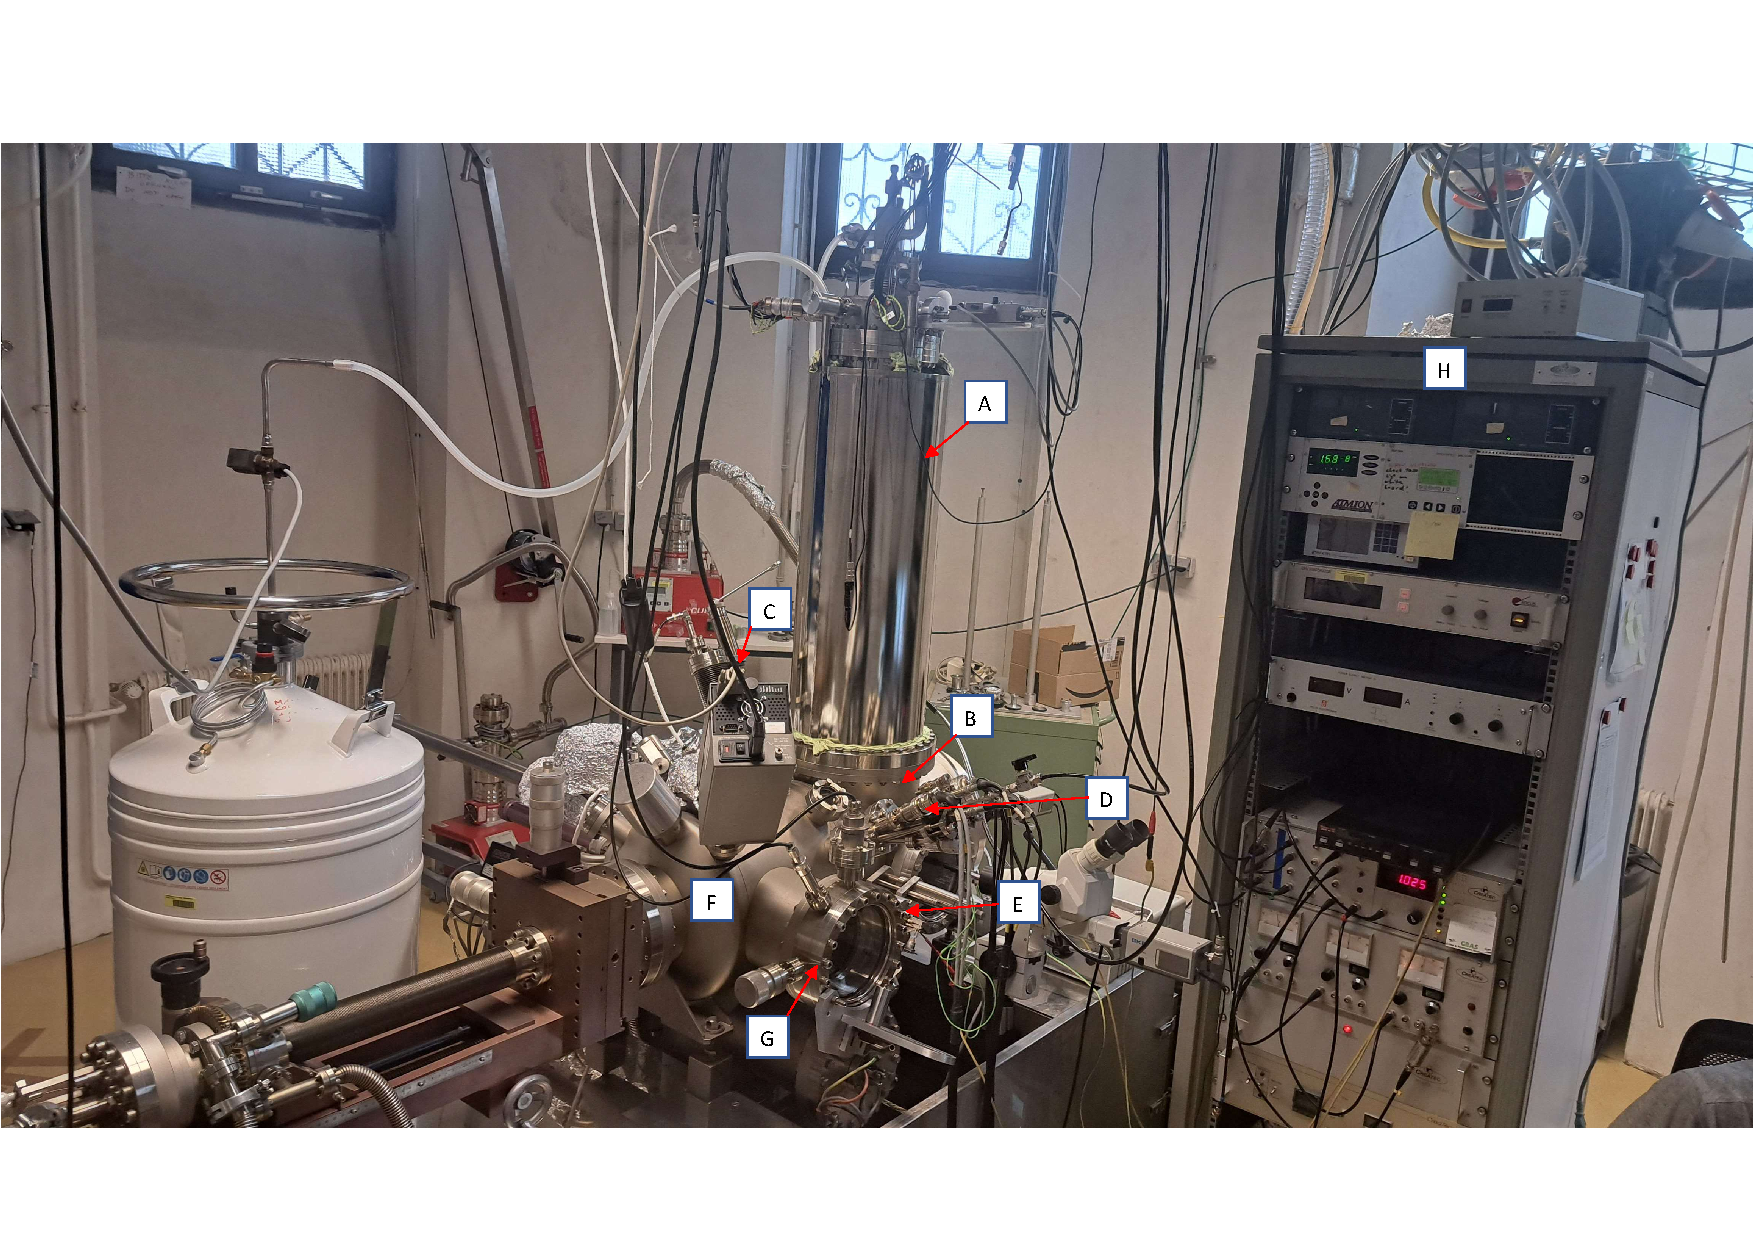
\includegraphics[width=0.9\textwidth]{Experimental_Setup/STM_Picture_1_edited.pdf}

The Probe-holder can be moved in each direction and rotated using an integrated arm in the PC.
It is also used to insert the Probe-holder into the MC.
The PC is equipped with a LEED system, which fluorescent screen can be extended. 
Additionally the PC has a metal-evaporator and organic-molecule evaporator (e-beam evaporator with a triple Knudsen cell) which are used to deposit submono- or monolayer structres onto an circular sample (10 mm x 2 mm).
This sample is mounted onto the previously mentioned Probe-holder, a Heatwaves Labs Inc. button heater with a resistive heating range of 20 K - 900 K.
The sample can also be cooled using LN2 or LHe through built-in pipe system in the manipulator arm.
A Quartz-Crystal Microbalance (QCM) with sub Angstöm precision is used to monitor the deposition thickness.
To clean the sample, an Argon sputter gun is employed, which utilizes an electric field to ionize and accelerate the argon gas.
The MC consists of a LT-STM which is surrounded by a two-shell cryostat, to which it is fixed, and two radiation shields to archieve temperatures as low as 7 K.
In this thesis the cryostat chamber was filled with LN2 which means it was oparated at 75 K.
The primary measuring unit (tip and sample storage place) is vibrationally damped using a coupled spring system.

%************AUSWERTUNG****************
\chapter{Results}
\label{sec:results}
sup
%************DISKUSSION***************
\chapter{Discussion}
\label{sec:Discussion}
seas


%\bibliography{literatur.bib}
%\bibliographystyle{seminarstyle}
\end{document}